\documentclass[titlepage,a4paper]{article}

\usepackage{a4wide}
\usepackage[colorlinks=true,linkcolor=black,urlcolor=blue,bookmarksopen=true]{hyperref}
\usepackage{bookmark}
\usepackage{fancyhdr}
\usepackage[spanish]{babel}
\usepackage[utf8]{inputenc}
\usepackage[T1]{fontenc}
\usepackage{graphicx}
\usepackage{float}

\pagestyle{fancy} % Encabezado y pie de página
\fancyhf{}
\fancyhead[L]{TP1S - Elvis CLAROS}
\fancyhead[R]{Algoritmos y Programación III - FIUBA}
\renewcommand{\headrulewidth}{0.4pt}
\fancyfoot[C]{\thepage}
\renewcommand{\footrulewidth}{0.4pt}

\begin{document}
\begin{titlepage} % Carátula
	\hfill
\includegraphics[width=6cm]{logofiuba.jpg}
    \centering
    \vfill
    \Huge \textbf{Trabajo Práctico 1 — Smalltalk}
    \vskip2cm
    \Large [7507/9502] Algoritmos y Programación III\\
    Curso 2 \\ % Curso 1 para el de la tarde y 2 para el de la noche
    Segundo cuatrimestre de 2019 
    \vfill
    \begin{tabular}{ | l | l | } % Datos del alumno
      \hline
      Alumno: & CLAROS, Elvis \\ \hline
      Número de padrón: & 99879 \\ \hline
      Email: & eclaros@fi.uba.ar \\ \hline
  	\end{tabular}
    \vfill
    \vfill
\end{titlepage}

\tableofcontents % Índice general
\newpage

\section{Introducción}\label{sec:intro}
El presente informe reúne la documentación de la solución del primer trabajo práctico de la materia Algoritmos y Programación III que consiste en desarrollar una aplicación de un sistema de chat en Pharo utilizando los conceptos del paradigma de la orientación a objetos vistos hasta ahora en el curso.

\section{Supuestos}\label{sec:supuestos}
% Deberá contener explicaciones de cada uno de los supuestos que el alumno haya tenido que adoptar a partir de situaciones que no estén contempladas en la especificación.

Entre los \textbf{supuestos} encontrados esta si una \textbf{conversación} se puede dar entre cero personas, en mi modelo se toma como posible esa opción ya que si al momento de crear una conversación se le pasa usuarios (o usuario) que no pertenece la conversación va a ser creado de todas formas.\\Otra supuesto que se cruzo en mi camino es, que hacer cuando se pide resumir una notificación del usuario o un mensaje de algún canal a una longitud menor a la del mensaje mismo. En este caso se opto por no permitir esa situación.\\
También me encontré con la situación de que pasa si un usuario determinado no se encuentra en \\textbf{AlgoChat}, se tomo la decisión de producir una excepciona.\\ Todo lo anteriormente mencionado serian los principales supuestos que se me presentaron.


\section{Modelo de dominio}\label{sec:modelo}
% Explicación concisa del diseño general del trabajo.
\begin{description}
\item[AlgoChat] Es la clase principal; la cual delega de forma completa todos sus mensaje, esta diseñada para trabajar con el enunciado del \\textbf{TP1}.
\item[Usuario] Esta clase es factible a recibir y guardar los mensajes y las palabras claves. \\Responde las notificaciones sin resumir y de forma resumida.\\
También recibe la responsabilidad de notificarse así mismo si es mencionado o mencionan alguna de sus palabras claves en el alguna publicación en los canales.

\item[Canal] Esta clase recibe y guarda sus mensajes. Una vez que recibió un mensaje, pasa el mensaje a los usuarios que se le suscribieron por si son mencionados o alguna de sus palabras clave aparece para que estos se notifiquen si corresponde.

\item[PalabraClave] Su función principal es la de saber para cual canal esta pausado. Pero también puede cambiar su estado a pausado para un determinado canal y también reanuda si un determinado si tenia el estado pausado para un determinado canal.
\item[Conversacion] La clase cumple con guardar los mensajes que se le enviaron y repartirlo entre los usuarios que la conforman.
\end{description}

\section{Diagramas de clase}\label{sec:diagramasdeclase}
% Uno o varios diagramas de clases mostrando las relaciones estáticas entre las clases.  Puede agregarse todo el texto necesario para aclarar y explicar su diseño. Recuerden que la idea de todo el documento es que quede documentado y entendible cómo está implementada la solución.

A continuación se presenta el \\textbf{Diagrama de Clases} mostrando la relación estática entre ellas.

\begin{figure}[H]
\centering
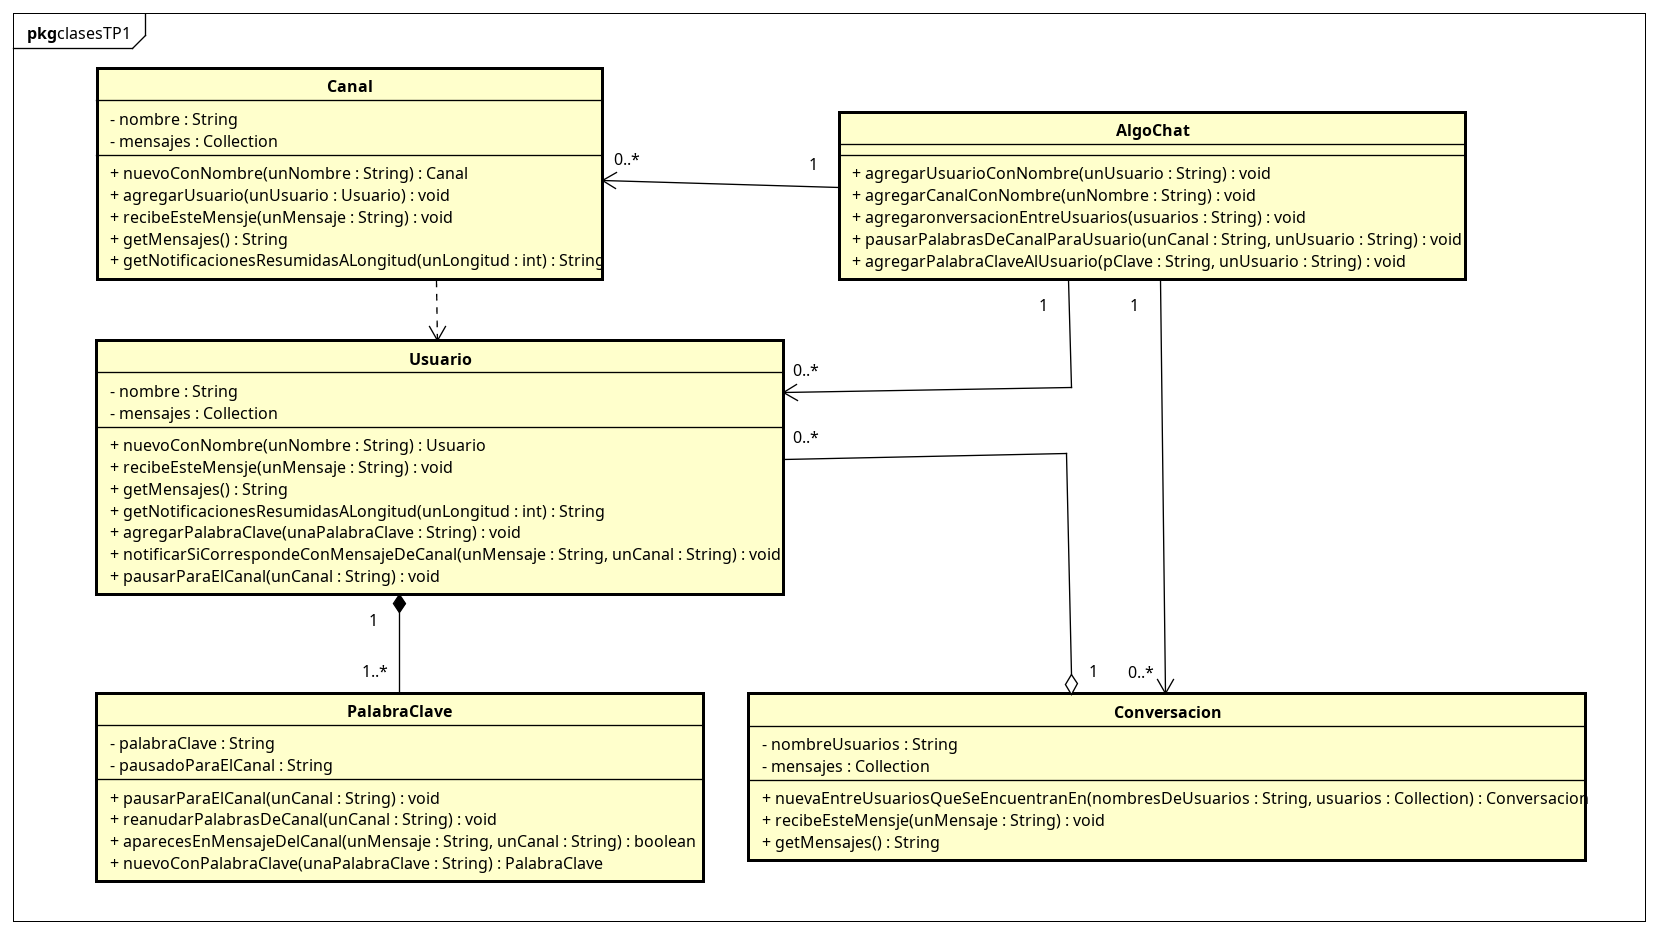
\includegraphics[width=0.8\textwidth]{DiagramaDeClasesTP1.png}
\caption{\label{fig:class01}Diagrama del AlgoChat.}
\end{figure}

\section{Detalles de implementación}\label{sec:implementacion}
% Explicaciones sobre la implementación interna de algunas clases que consideren que puedan llegar a resultar interesantes.

\subsection{AlgoChat}Es una clase central que delega la totalidad de sus mensajes.

\subsection{Usuario} Esta clase tiene un muy interesante protocolo, para su mensaje \\verb|notificarSiCorrespondeConMensaje: unMensaje deCanal: unCana| y es la siguiente:
\begin{verbatim}
notificarSiCorrespondeConMensaje: unMensaje deCanal: unCanal
((unMensaje findString: '@',nombre) > 0)  ifTrue:  [mensajes add: unMensaje] 
ifFalse: [
(palabrasClaves anySatisfy: [ 
:palabraClave | palabraClave aparecesEnMensaje: unMensaje delCanal: unCanal ]) 
ifTrue: [ mensajes add: unMensaje ] 
	]. 
\end{verbatim}
Se trato de buscar un modelo tal que la solución no parezca estructurada.
\subsection{Conversacion} Es una clase bastante sencilla ya que solo guarda los mensajes y cuando recibe un mensaje distribuí entre los usuarios que están en la conversación.
\subsection{PalabraClave} Uno de los principales problemas del TP1 fue el echo de modelar el mensaje\\ \verb|pausarPalabrasDeCanal: unCanal paraUsuario: unUsuario|\\ el cual termino delegada a esta clase (PalabraClave) y se lo modelo de la siguiente forma:
\begin{verbatim}
    aparecesEnMensaje: unMensaje delCanal: unCanal

((pausadoParaElCanal findString: unCanal) > 0)
ifTrue: [ ^ false ] ifFalse: [
^ ((unMensaje findString: palabraClave ) > 0)].
\end{verbatim}
Con esta linea \verb|(pausadoParaElCanal findString: unCanal) > 0)| se determina si esta pausada para unCanal, en caso de estar pausada la \verb|PalabraClave| retorna \verb|^false.| a pesar de aparecer en unMensaje.\\ De esta forma se modelo la solución para el mensaje \verb|pausarPalabrasDeCanal: unCanal paraUsuario: unUsuario|.
\subsection{Canal} Canal entre los mensajes que responde tiene recibir mensaje y notificar a los usuarios suscritos que son mencionados aparecen sus palabras clave se resuelve con la linea:
\begin{verbatim}
usuario notificarSiCorrespondeConMensaje: unMensaje deCanal: nombre
\end{verbatim}

De esta forma da la responsabilidad al usuario de guardar la notificación si es mencionado él o alguna de sus palabras claves. Como el usuario recibe también el nombre del canal y él (mejor dicho sus palabras claves saben) si están o no pausadas para ese canal.


%Quisque tempus, tortor et convallis interdum, ipsum leo tempus ipsum, in molestie tortor arcu sit amet tellus. Praesent fermentum hendrerit nulla. In maximus ornare maximus. Nullam consectetur placerat enim sit amet lacinia. Etiam pellentesque tellus consectetur hendrerit iaculis. Sed non laoreet felis.

\section{Excepciones}\label{sec:excepciones}
% Explicación de cada una de las excepciones creadas y con qué fin fueron creadas.

\begin{description}
\item[LongituDeUnMesajeMenorAlaLongitudAResumirError] Es lanzada cuando se trata de reducir un mensaje a una longitud menor que la suya la usan las Clases Usuario y Canal se implemento mas que todo para dar claridad a la excepción que es lanzada por el mensaje \\textbf{first:} que usada para reducir el mensaje.
\item[NombreNoSeEncuentraError] La excepción da aviso cuando usuario o canal no se encuentra. La finalidad es que se ponga en evidencia que el usuario (o canal) al que se le quiere por ejemplo mandar un mensaje, no exista (o no pertenezca) .
%\item[Excepcion] Integer porta efficitur felis. Etiam facilisis consectetur sem, ac efficitur orci. Nam a ante commodo, fringilla nisl a, sollicitudin est.
%\item[Excepcion] Aliquam erat volutpat. Fusce quis efficitur augue. Fusce egestas mauris a nisi finibus volutpat. Maecenas venenatis ligula ut nisi maximus, vel ultricies enim scelerisque.
%\item[Excepcion] Mauris gatis feugiat erat non euismod. Donec sagittis orci enim, et convallis lacus sodales at. Nunc laoreet leo vel metus eleifend, vel aliquam sem tincidunt. Nunc imperdiet eget erat eget tincidunt. Morbi tempus risus quis nulla faucibus facilisis. Sed varius nunc vel neque rutrum vestibulum.
\end{description}

\section{Diagramas de secuencia}\label{sec:diagramasdesecuencia}
% Mostrar las secuencias interesantes que hayan implementado. Pueden agregar texto para explicar si algo no queda claro.
Contención se describen algunas secuencias. 
En la Figura ~\ref{fig:seq02} se puede observar la secuencia que se sigue para que \verb|AlgoChat| pueda pausar una palabra para un canal donde cierto usuario pertenece.
\begin{figure}[H]
\centering
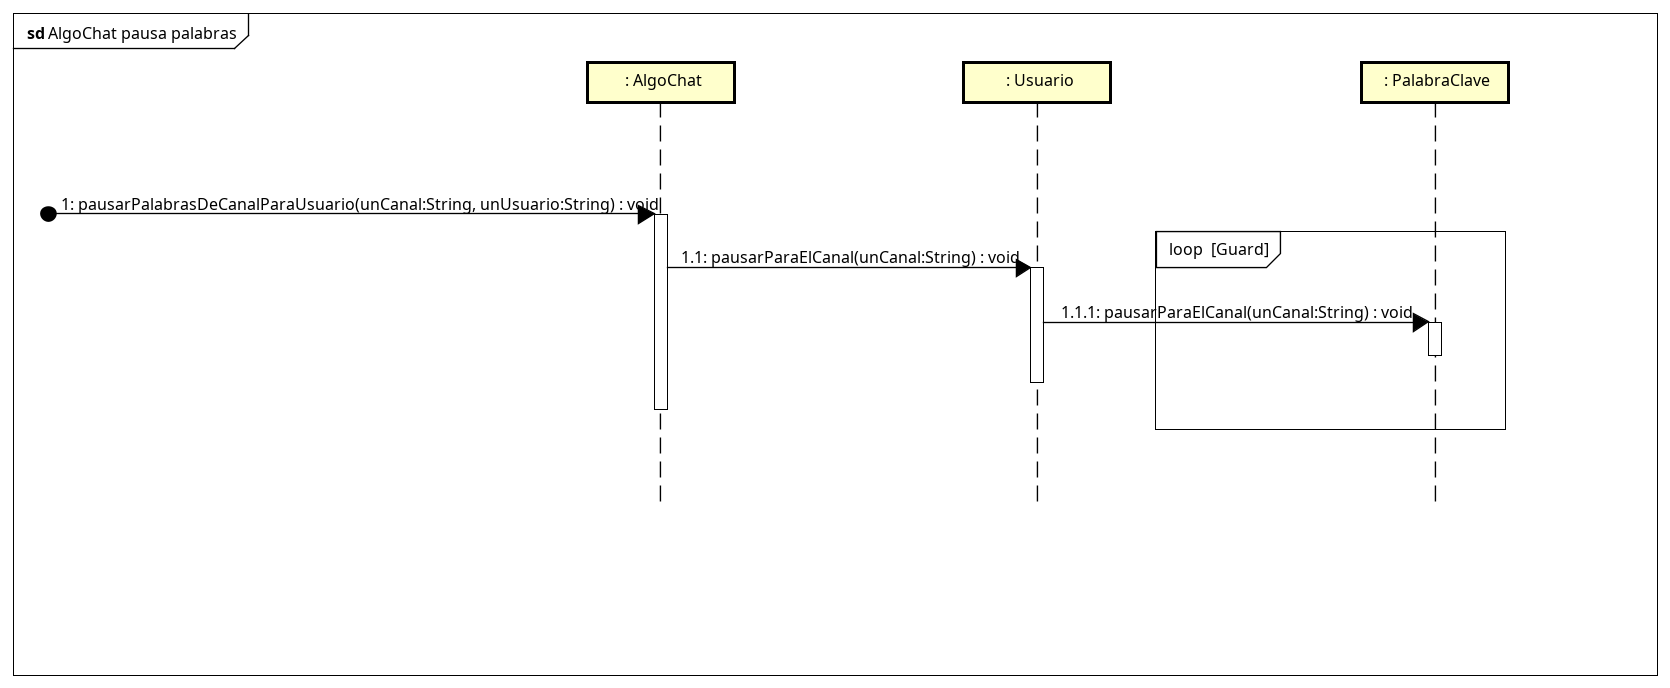
\includegraphics[width=\textwidth]{AlgoChat_pausa_palabras.png}
\caption{\label{fig:seq02}AlgoChat pausa palabra clave.}
\end{figure}

En esta Figura ~\ref{fig:seq03} se puede ver la delegación que realiza \verb|Canal| a la clase \verb|Usuario|, por tener esta última mucho más recursos para poder resolverlo fácilmente.
\begin{figure}[H]
\centering
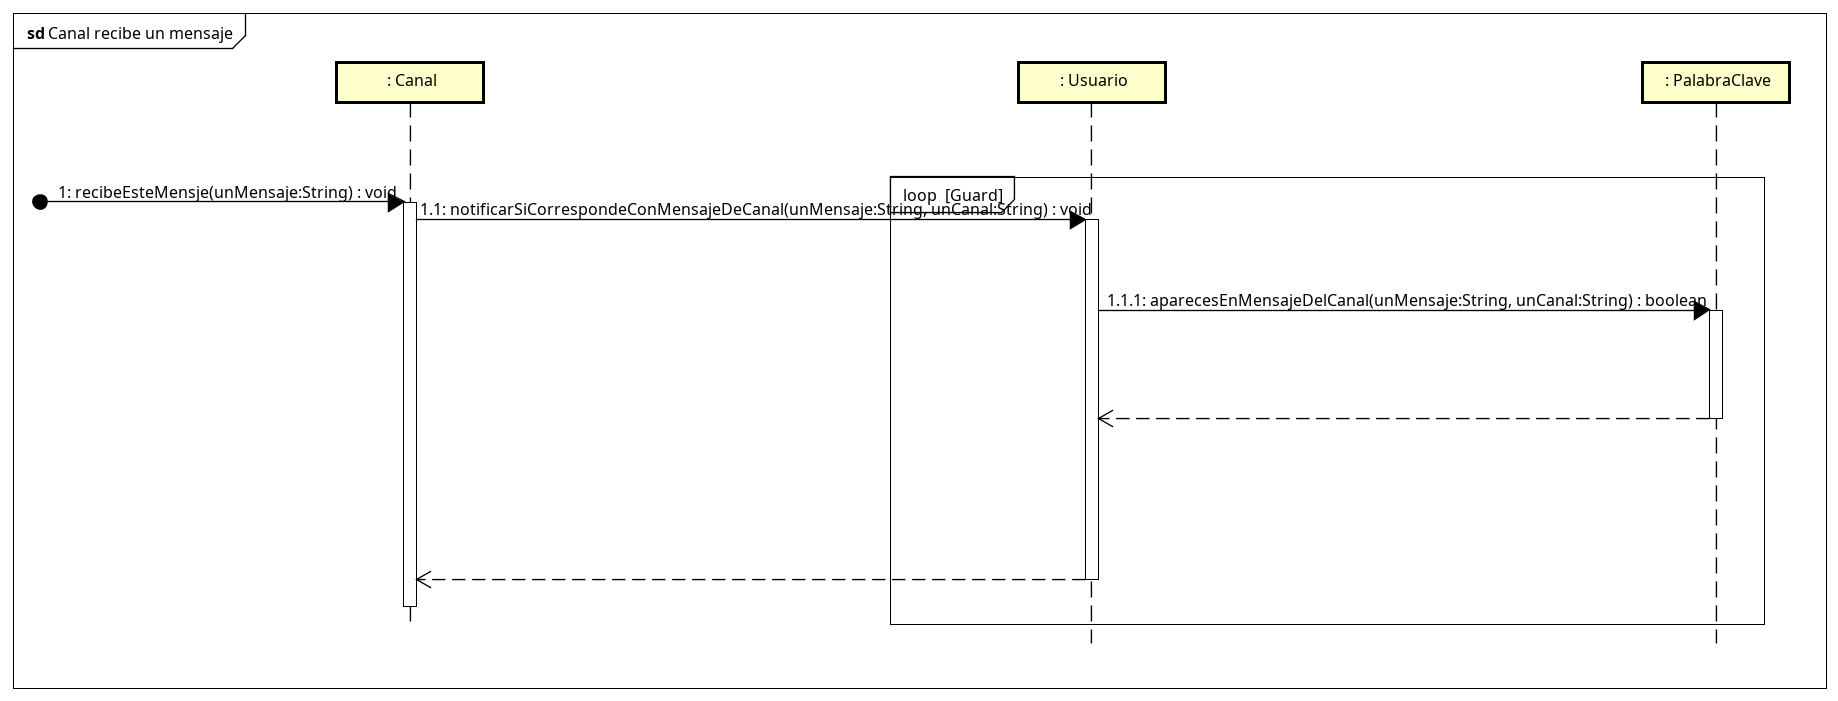
\includegraphics[width=\textwidth]{Canal_recibe_un_mensaje.png}
\caption{\label{fig:seq03}Canal recibe un mensaje.}
\end{figure}
En este ultima Figura (Figura ~\ref{fig:seq04}) se pretende ilustrar la instanciación de la clase \verb|PalabraClave|, como se puede observar ésta es instanciada por \verb|Usuario|.\\\verb|PalabraClave| y \verb|Usuario| tienen una relación muy estrecha ya que la existencia de la primera no tendría sentido sin la segunda.
\begin{figure}[H]
\centering
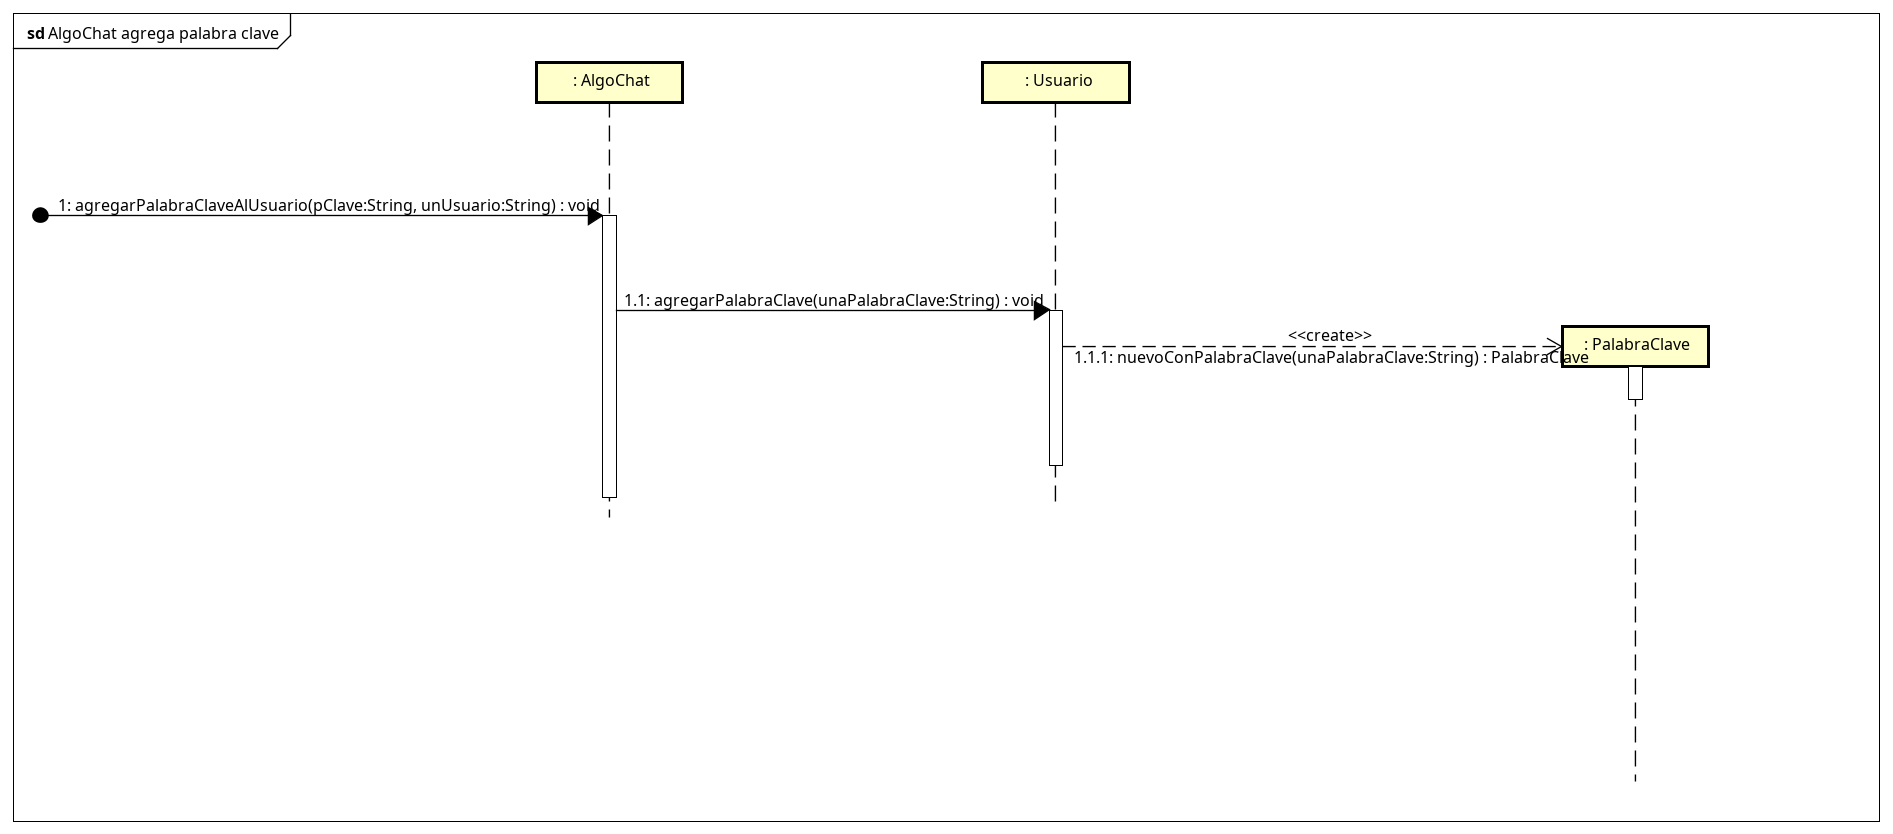
\includegraphics[width=0.8\textwidth]{AlgoChat_agrega_palabra_clave.png}
\caption{\label{fig:seq04}AlgoChat agrega palabra clave.}
\end{figure}

\end{document}
